\section{Antecedentes}
\subsection{Crecimiento de la población de adultos mayores}

De acuerdo con la OMS, a todo individuo mayor de 60 años se le llamará de forma imperceptible persona de la tercera edad. Las personas de 60 años de edad o mayores realizan aportaciones valiosas a la sociedad como miembros activos de la familia, voluntarios y participantes dinámicos en la fuerza de trabajo. Por otra parte, a medida que se envejece aumentan las probabilidades de padecer varias afecciones al mismo tiempo. \\

\begin{itemize}
	\item La población mundial está envejeciendo rápidamente. Entre 2015 y 2050 la proporción de la población mundial mayor de 60 años se multiplicará casi por dos, pasando del 12\% al 22\%.
	\item Los trastornos neuropsiquiátricos representan el 6,6\% de la discapacidad total, años de vida ajustados en función de la discapacidad (AVAD) en este grupo etario.
\end{itemize}

En números absolutos, el aumento previsto es de 900 millones a 2 000 millones de personas mayores de 60 años. Además de las causas generales de tensión con que se contrarresta todo el mundo, muchos adultos mayores se ven privados de la capacidad de vivir independientemente por dificultades de movilidad, dolor crónico, fragilidad u otros problemas mentales o físicos, de modo que necesitan asistencia a largo plazo. Además, entre los ancianos son más frecuentes experiencias como el dolor por la muerte de un ser querido, un descenso del nivel socio-económico como consecuencia de la jubilación, o la discapacidad \cite{cuatro}.

\subsection{Discapacidades en los adultos mayores}

Publicaciones avaladas por las distintas asociaciones en diferentes países (Encuesta Nacional sobre el Uso del Tiempo (ENUT), Instituto Nacional de las Mujeres (INMUJERES), el Fondo de las Naciones Unidas para el Desarrollo de la Mujer (UNIFEM), el Programa de las Naciones Unidas para el Desarrollo (PNUD) y el Instituto Nacional de Estadística y Geografía (INEGI)), han dedicado recursos a la elaboración de encuestas del uso del tiempo, para conseguir información sobre la forma como las personas dividen su tiempo en realizar diversas actividades, como trabajar, estudiar, divertirse, comer y descansar, entre otras; y de manera específica, el tiempo que dedican al trabajo doméstico (cocinar, limpiar, lavar la ropa), así como a realizar las compras, pagar servicios, atender a los hijos, etcétera. Para este trabajo nos enfocamos solo al uso del tiempo destinado al cuidado de los adultos mayores considerando que es un problema reflejado en la economía familiar, debido a que personas de este grupo son susceptibles de sufrir alguna discapacidad, requiriendo la atención por parte de personal especializado, como enfermeras, o la ayuda de familiares. \\ 

De las personas de 60 años y más, que registró la Encuesta Nacional sobre el Uso del Tiempo (ENUT) 2009 como necesitadas de cuidado, 59\% fueron mujeres y 41\% hombres. Las razones de cuidado no difieren de manera notable por sexo. Un 74.8\% lo clasificó como necesidades de cuidado continuo (55.9\% debido a que tenía alguna enfermedad crónica y 18.9\% por tener alguna limitación física o mental), mientras que el restante 39.5\% fue por causa de una enfermedad temporal. \\

En los resultados de la gráfica 1.1 se aprecia considerablemente mayor el número de mujeres que de hombres que requieren de cuidado. Hay que resaltar que más de medio millón de personas adultas mayores requieren de cuidados continuos debido a una limitación física o mental. Necesidades de cuidado según datos de la Encuesta Nacional sobre Uso del Tiempo (ENUT) 2009, 25.3\% de las personas adultas mayores, 27.8\% de las mujeres y 22.5\% de los hombres necesitaron que alguna persona de su hogar le brindará cuidados o apoyo. Como era de esperarse, las necesidades de cuidado se incrementan conforme aumenta la edad \cite{cinco}.

\begin{figure}[h]
	\centering
	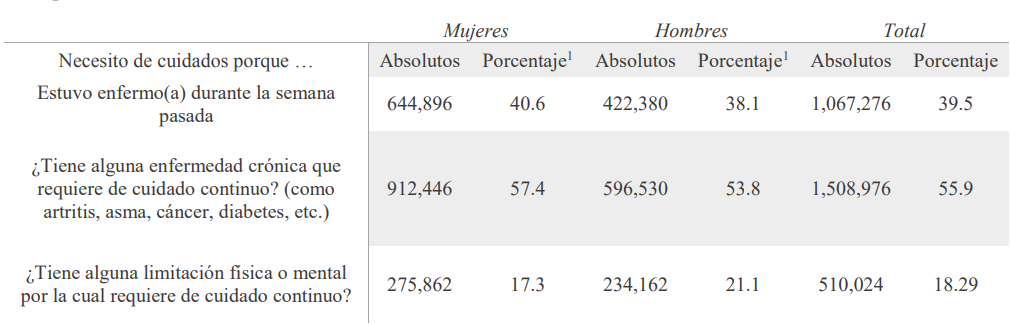
\includegraphics[scale=0.47]{introduccion/imagenes/grafica1_1}
	\textbf{\caption{\small{Población de 60 años o más que necesitó de cuidados la semana previa a la entrevista de la ENUT 2009 por su sexo, según clasificación de cuidado \cite{cinco}.}}}
	\label{FiguraSeccion1.1.2:1.1}
\end{figure}

\subsection{Discapacidad visual}

Hoy en día la discapacidad visual es cada vez mayor y esto se ve reflejado en la población de 50 años o más, por tanto, este tipo de limitación provoca la disminución o pérdida de las funciones visuales, lo cual implica que las personas participen cada vez menos en las actividades cotidianas. \\

\begin{figure}[h]
	\centering
	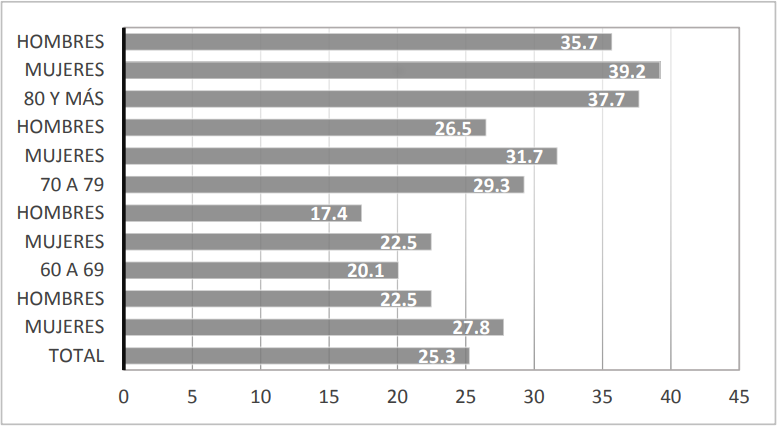
\includegraphics[scale=0.47]{introduccion/imagenes/grafica1_2}
	\textbf{\caption{\small{Porcentaje de población adulta mayor que necesitó cuidados en el hogar por grupo de edad y sexo, 2009 \cite{cinco}.}}}
	\label{FiguraSeccion1.1.2:1.2}
\end{figure}

El 82\% de las personas que padecen ceguera tienen 50 años o más. Con arreglo a la Clasificación Internacional de Enfermedades (CIE-10, actualización y revisión de 2006), la función visual se subdivide en cuatro niveles:

\begin{itemize}
	\item Visión normal.
	\item Discapacidad visual moderada.
	\item Discapacidad visual grave.
	\item Ceguera.
\end{itemize}

Principales causas de discapacidad visual:

\begin{itemize}
	\item Errores de refracción (miopía, hipermetropía o astigmatismo) no corregidos: 43\%.
	\item Cataratas no operadas: 33\%.
	\item Glaucoma: 2\%.
\end{itemize}

Alrededor de un 65\% de las personas con discapacidad visual son mayores de 50 años, si bien este grupo de edad apenas representa un 20\% de la población mundial. Con una población anciana en aumento en muchos países, más personas estarán en riesgo de sufrir discapacidad visual por enfermedades oculares crónicas y envejecimiento \cite{seis}.

\subsection{Discapacidad auditiva}

Otra de las discapacidades que se presenta en las personas mayores es la pérdida de audición, dado que cuando las personas empiezan a envejecer se puede presentar este tipo de limitación, por tanto esta función es muy esencial para el ser humano debido a que es fundamental para la plena interacción con la sociedad. \\

El oído es un órgano muy complicado y a la vez importante puesto que la pérdida de audición puede causar problemas para comunicarse con los demás, también se ven afectados para el pleno desarrollo tanto personal como emocional entre otros. \\

Los problemas de comunicación y el acceso limitado a los servicios pueden tener efectos importantes en la vida cotidiana y generar sensación de soledad, aislamiento y frustración, sobre todo en las personas mayores que padecen pérdida de audición. \\
Por sordera y pérdida de audición se entiende una pérdida de audición superior a 40dB en el oído con mejor audición en los adultos. Más del 5\% de la población mundial (360 millones de personas) padece pérdida de audición (328 millones de adultos y 32 millones de niños). Aproximadamente una tercera parte de las personas mayores de 65 años padece pérdida de audición \cite{siete}.

\subsection{Demencia}

Dado que la demencia es consecuencia natural del envejecimiento, podemos decir que el principal órgano que se ve afectado es el cerebro, por ello es una de las principales causas de discapacidad en el mundo que generan dependencia a medida que tiene un impacto tanto físico, psicológico, social y económico en los cuidadores, las familias y la sociedad. \\

La demencia es un síndrome que implica el deterioro de la memoria, el intelecto, el comportamiento y la capacidad para realizar actividades de la vida diaria, afectando principalmente a la personas mayores. Se calcula que en el mundo hay unos 47,5 millones de personas aquejadas de demencia. Se prevé que el número de estas personas aumentará a 75,6 millones en 2030 y a 135,5 millones en 2050; además, la mayoría de esos pacientes vivirán en países de ingresos bajos y medianos \cite{ocho}.

\subsection{Caídas}

La edad es uno de los principales factores de riesgo de las caídas. Los ancianos son quienes corren mayor riesgo de muerte o lesión grave por caídas, y el riesgo aumenta con la edad. La magnitud del riesgo puede deberse, al menos en parte, a los trastornos físicos, sensoriales y cognitivos relacionados con el envejecimiento, así como a la falta de adaptación del entorno a las necesidades de la población de edad avanzada. \\

Otros factores de riesgo son:

\begin{itemize}
	\item Trastornos médicos subyacentes, tales como trastornos neurológicos, cardíacos u otras afecciones incapacitantes.
	\item Efectos colaterales de los medicamentos, inactividad física y pérdida de equilibrio, sobre todo en las personas mayores.
	\item Problemas cognitivos, visuales y de movilidad, especialmente entre quienes viven en instituciones tales como las residencias de ancianos o los centros de atención a pacientes crónicos. 
\end{itemize}

Las caídas se definen como acontecimientos involuntarios que hacen perder el equilibrio y dar con el cuerpo en tierra u otra superficie firme que lo detenga. Las lesiones relacionadas con las caídas pueden ser mortales, aunque la mayoría de ellas no lo son. \\

\begin{itemize}
	\item Las caídas son la segunda causa mundial de muerte por lesiones accidentales o no intencionales.
	\item Los mayores de 65 años son quienes sufren más caídas mortales.
	\item Cada año se producen 37,3 millones de caídas cuya gravedad requiere atención médica.
\end{itemize}

Las mayores tasas de mortalidad por esta causa corresponden en todas las regiones del mundo a los mayores de 60 años. Cada año se producen 37,3 millones de caídas que, aunque no sean mortales, requieren atención médica y suponen la pérdida de más de 17 millones de años de vida ajustados en función de la discapacidad (AVAD). La mayor morbilidad corresponde a los mayores de 65 años, sin embargo, quienes padecen discapacidad a causa de las caídas, y en particular los ancianos, corren más riesgo de necesitar atención a largo plazo e ingreso en alguna institución \cite{nueve}.